\section{Le jeu de Lola (3 points bonus)}

Lola propose un jeu à ses deux amis, Juliette et Aurèle.

\begin{center}
	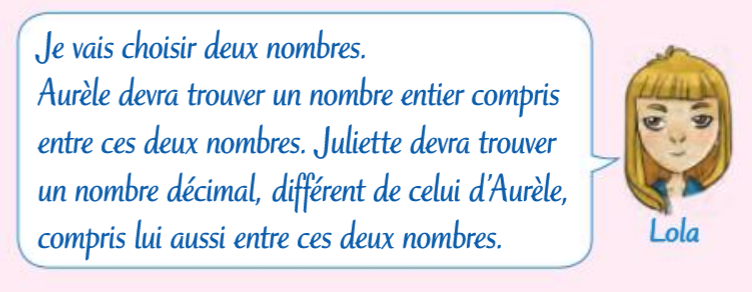
\includegraphics[scale=0.7]{img/lola}
\end{center}

\begin{questions}
	\question[1] Lola a choisi  \num{322.1} et \num{325.4}. Donner toutes les réponses possibles pour Aurèle et dix réponses possibles pour Juliette.
	
	\begin{solution}
		Les réponses possibles pour Aurèle sont 323, 324 et 325. \\
		
		Juliette peut répondre, entre autres \num{322.15}; \num{322.35}; \num{322.55}; \num{322.8}; \num{323.005}; \num{323.735}; \num{323.964}; \num{324.1024} ; \num{325.2048} et \num{325.399999}.
	\end{solution}
	
	\question[1] Lola choisi tà présent \num{12.3} et \num{12.4}. Donner toutes les réponses possibles pour Aurèle et dix réponses possibles pour Juliette. Peut-on donner toutes les réponses possibles ?
	\begin{solution}
		Il n'y a pas de réponse possible pour Aurèle il n'y aucun nombre entier compris entre \num{12.3} et \num{12.4}.\\
		
		Juliette peut répondre, entre autres \num{12.31}; \num{12.311}; \num{12.3111}; \num{12.31111}; \num{12.311111}; \num{12.3111111}; \num{12.31111111}; \num{12.311111111} ; \num{12.3111111111} et \num{12.31111111111}.\\
		
		Il n'est pas possible de donner toutes les réponses possibles pour Juliette il y a en une infinité.
	\end{solution}
	
	
\question[1] Aurèle n'est pas content et dit à Lola que ses règles du jeu sont injustes. Expliquer pourquoi.

\begin{solution}
	Quels que soient les nombres choisis par Lola, Aurèle aura toujours un nombre limité de réponses possible et Juliette une infinité de possibilités.
\end{solution}
\end{questions}